% FADE: Rethinking Sequential Recommendation as Filter-Augmented Dense Retrieval
% Built on the Springer LLNCS template (Latex-Template-for-Springer.zip).
% Converted from paper_draft.md -- see that file for the source-of-truth prose
% and paper_outline.md for the decisions behind each section.
\documentclass[runningheads]{llncs}
%
\usepackage[T1]{fontenc}
\usepackage[utf8]{inputenc}
\usepackage{graphicx}
\usepackage{amsmath}
\usepackage{amssymb}
\usepackage{booktabs}
\usepackage{float}
\DeclareMathOperator*{\argmax}{arg\,max}
%
% If you use the hyperref package, please uncomment the following two lines
% to display URLs in blue roman font according to Springer's eBook style:
%\usepackage{color}
%\renewcommand\UrlFont{\color{blue}\rmfamily}
%\urlstyle{rm}
%
\begin{document}
%
\title{FADE: Rethinking Sequential Recommendation as Filter-Augmented Dense Retrieval}
%
\titlerunning{FADE: Filter-Augmented Dense Retrieval for Sequential Recommendation}
%
\author{Nguyen Do Hai\inst{1,2}\orcidID{0009-0009-8496-6905} \and \\  Tu Minh Phuong\inst{2}\orcidID{0000-0001-6415-228X}}
%
\authorrunning{N. D. Hai and T. M. Phuong}
%
\institute{People's Security Academy, Hanoi, Vietnam\\
\email{nguyendohai@gmail.com}\\ \and
MLA Lab, Posts and Telecommunications Institute of Technology, Hanoi, Vietnam\\
\email{phuongtm@ptit.edu.vn}}
%
\maketitle
%
\begin{abstract}
Sequential recommendation (SR) aims to predict what a user will interact with next by modeling the order of their past behavior. Large language models (LLMs) have recently been applied to SR in a variety of ways, and formulating SR as an LLM-based information-retrieval (IR) problem, in which a user's recent interaction history is converted into a text query and matched against candidate items treated as documents in a retrieval corpus, is one such promising direction pursued by a growing body of prior work. Applying LLM-based IR to SR, however, raises three challenges that prior work in this space has not fully resolved. First, jointly encoding every candidate item with the query via a cross-encoder is too costly at catalog scale, making a bi-encoder close to a necessity. Second, the leave-one-out protocol standard in SR supplies only one training example per user, far too little to fine-tune an LLM-scale encoder. Third, because the query is built directly from previously-consumed item text, such retrievers tend to repeatedly rank those same items at the top of the list. We present FADE (Filter-Augmented Dense rEtrieval), which addresses these three challenges respectively with a Bi-Encoder Dense Retrieval applied systematically to SR, sliding-window data augmentation that recovers the missing per-position supervision, and a lightweight, training-free filter that removes previously-consumed items from the ranked list. Experiments on three real-world datasets show that FADE substantially outperforms prior LLM-based information-retrieval approaches to sequential recommendation.

\keywords{Sequential Recommendation \and Dense Retrieval \and Fine-tuning LLM \and Information Retrieval}
\end{abstract}
%
%
%
\section{Introduction}
\label{sec:intro}

Sequential recommendation (SR) predicts the next item a user will interact with from their chronological interaction history, which is used to model the user's preference. Early work modeled this ordering with Markov chains, assuming the next action depends only on the last one or few; later architectures relaxed this local assumption while pursuing the same underlying goal of exploiting sequence order, whether through a recurrent network (GRU4Rec~\cite{hidasi2016}), a graph neural network over the session (SR-GNN~\cite{wu2019}), or self-attention over the sequence (SASRec~\cite{kang2018}). All of these represent items purely as trainable ID embeddings learned end-to-end from the interaction matrix, with no access to any information about what an item actually is. The recent rise of large language models (LLMs) has opened a complementary direction: instead of learning item identity from scratch, an LLM can encode the textual side information already available for most catalogs, such as titles, descriptions, and categories, bringing broad semantic and world knowledge that pure ID-based collaborative filtering has no access to.

One increasingly popular way to apply this idea is to represent SR as an information retrieval (IR) problem. A user's recent interaction history is converted into a text query, the item set becomes a document corpus, and predicting the next item reduces to retrieving the item most similar to the query in a learned embedding space. Figure~\ref{fig:example}(a) illustrates this on Amazon Beauty: given a query built from a user's three most recent purchases, namely a sunscreen, a facial cleanser, and a treatment serum, an effective retriever should rank a moisturizing cream highest, not because any user in the training data ever bought exactly this sequence before (there may be no such co-occurrence anywhere in the data), but because the retriever's embedding space captures that a moisturizer is the natural next step in a skincare routine. This is precisely the appeal of the retrieval reformulation over ID-based collaborative filtering: relevance is judged by \emph{semantic} similarity of text rather than by \emph{statistical co-occurrence} of item identifiers, letting the model generalize to item combinations it has never observed.

\begin{figure}
    \centering
    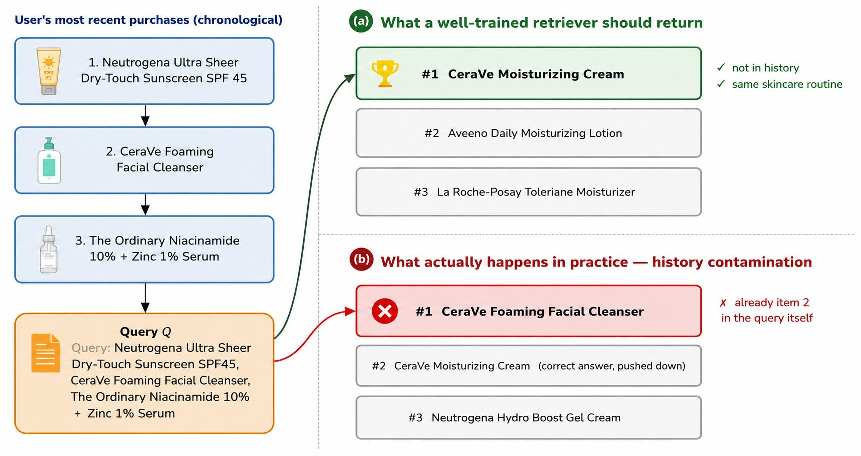
\includegraphics[width=0.75\linewidth]{fig1_introduction_example.pdf}
    \caption{Illustrative example on Amazon Beauty. (a) A well-trained retriever ranks a novel, relevant
item first; (b) an unfiltered retriever instead re-surfaces an already-consumed item, an instance
of \emph{seen-item bias}}
    \label{fig:example}
\end{figure}

Despite this appeal, applying LLM-based dense retrieval to SR raises three challenges specific to the recommendation setting. First, scoring relevance with an LLM does not by itself dictate \emph{how} query and candidate items should be encoded. The most accurate option would be to jointly encode each (query, candidate) pair with full cross-attention, as a cross-encoder does, but this is computationally infeasible for the retrieval stage itself: an item set can contain tens of thousands to millions of items, and re-running a full LLM forward pass over every candidate for every query is prohibitive at serving time. A \textbf{bi-encoder}, which encodes queries and documents independently so that item embeddings can be computed once offline and queried via approximate nearest-neighbor search, is therefore not merely a design preference inherited from prior text-retrieval work; it is close to a necessary condition for LLM-based retrieval to be practical at recommendation scale. Second, the standard leave-one-out training protocol used in SR provides very little supervision per user: with only the final interaction held out for testing, each user contributes exactly one (query, next-item) training pair by default. This is a poor match for fine-tuning an LLM-scale encoder, which typically needs substantially more examples than the handful one gets by directly borrowing this protocol from ID-based SR without adaptation. Third, because the query is built directly from the titles of previously-consumed items, a retriever trained with a standard contrastive objective tends to rank those same items, or items with near-identical titles, near the top of the result list, largely due to lexical overlap between the query and candidate text rather than genuine relevance. Figure~\ref{fig:example}(b) illustrates this for the same example as above: the already-purchased facial cleanser outranks the moisturizing cream, which is pushed down to rank~2. We refer to this pattern as \textbf{seen-item bias}.

We address these challenges with \textbf{FADE} (\textbf{F}ilter-\textbf{A}ugmented \textbf{D}ense r\textbf{E}trieval), a bi-encoder retriever for sequential recommendation built on a fine-tuned LLM backbone. FADE augments training with sliding-window sub-sequences to recover the per-position supervision that causal architectures such as SASRec obtain for free, and applies a lightweight, training-free history filter that removes previously-consumed items from the ranked list. Across three real-world datasets spanning short and long interaction histories, and at two backbone scales, FADE substantially outperforms both strong ID-based baselines and prior LLM-based
recommenders.

Our contributions are as follows:

\begin{itemize}
\item We apply a bi-encoder LLM retriever to sequential recommendation, adapting it to a setting where a multi-item query is matched against single-item documents.
\item We identify and mechanistically explain \emph{seen-item bias}, a retrieval-specific bias in which previously-consumed items dominate the ranked list, and fix it with a training-free filter.
\item We introduce sliding-window data augmentation for bi-encoder SR training, framed as recovering the per-position supervision that causal architectures obtain implicitly, and show it contributes substantially across all three datasets.
\item We conduct comprehensive experiments against ID-based baselines (GRU4Rec, SASRec, SR-GNN) and, where available, literature-reported LLM-based baselines, on three real-world datasets.
\end{itemize}

\section{Related Work}
\label{sec:relwork}

\paragraph{Sequential recommendation.}
Classical SR models predict the next item from a user's interaction sequence by learning item-ID embeddings end-to-end from interaction data alone: GRU4Rec models the sequence with a gated recurrent network~\cite{hidasi2016}, SR-GNN represents a session as a graph and applies a gated graph neural network~\cite{wu2019}, and SASRec replaces both with self-attention under a causal mask~\cite{kang2018}. All three condition purely on interaction order and item identity, without using any textual content, so they have no way to relate two items that never co-occur in the training data, however similar their content, and no natural way to reason about items outside the ID vocabulary seen during training. This is exactly the limitation that motivates representing SR as a text-retrieval problem instead, where relevance is judged by content rather than by co-occurrence statistics alone. We use all three as ID-based baselines in our experiments.

\paragraph{LLM-based sequential recommendation.}
A growing body of work applies LLMs to SR through approaches distinct from FADE's dense-retrieval reformulation. \emph{Generative retrieval} methods discard embedding-based ANN search entirely and instead train a model to directly generate an item's identifier: TIGER~\cite{rajput2023} quantizes each item's content embedding into a short sequence of discrete ``Semantic ID'' tokens via residual quantization, then trains a sequence-to-sequence model to autoregressively predict the target item's Semantic ID; ActionPiece~\cite{hou2025} improves on TIGER's tokenization by merging item-feature tokens based on their co-occurrence context, rather than tokenizing every item identically regardless of the sequence it appears in. \emph{LLM-as-ranker} methods keep a separate, lightweight candidate retriever and use the LLM only to re-rank its output: LlamaRec \cite{yue2023} does this in a single forward pass, via a verbalizer that reads a probability distribution over candidate items directly off the LLM's output logits rather than generating text. Other work integrates LLMs more tightly with existing ID-based architectures rather than replacing them: E4SRec~\cite{li2024} uses an LLM as a sequence encoder feeding into an ID-embedding prediction head, and EAGER-LLM~\cite{hong2025} injects collaborative (``exogenous'') signals into a decoder-only LLM recommender alongside its native semantic understanding, addressing a mismatch between an LLM's linguistic pretraining and the collaborative patterns recommendation requires. P5 \cite{geng2022} takes a different unification angle, casting many recommendation tasks, not only next-item prediction, as a single text-to-text, prompt-based objective. Closest to FADE is GLoSS~\cite{acharya2025}, which shares the same bi-encoder dense-retrieval architecture, matching a query embedding against embeddings of every candidate item. GLoSS, however, uses the LLM only to fine-tune the query side: a fine-tuned generator produces a text description of the item it predicts the user will buy next, and this description, together with every candidate item, is embedded by a separate bi-encoder (e5-small-v2~\cite{wang2022e5}) that is kept frozen rather than fine-tuned for retrieval.

\paragraph{Dense retrieval bi-encoders.}
Reformulating retrieval as independent query/document encoding followed by a shallow similarity comparison, the bi-encoder architecture was popularized in open-domain question answering by DPR~\cite{karpukhin2020}, which trains two separately-parameterized BERT encoders, and later adapted to an LLM-scale backbone by RepLLaMA~\cite{ma2024}, which replaces the two BERT towers with a single, weight-shared LLaMA-2 decoder and [EOS]-token pooling in place of [CLS] pooling. An aggregated, multi-item query matched against single-item documents is a pattern that appears elsewhere too, generally resolved with untied rather than shared encoders: conversational dense retrieval faces the same shape of problem, since a query built by concatenating several turns of dialogue history must be matched against single-passage documents, and ConvDR~\cite{yu2021} addresses it with a dedicated query encoder trained to imitate a separately-encoded, frozen document index; industrial two-tower recommender systems face it as well, aggregating a user's behavioral signals in one tower and a single item's content features in the other~\cite{yi2019}, again with two independently-parameterized towers.

\paragraph{Data augmentation.}
Generating multiple training instances from a single interaction sequence by sliding a fixed-size window across it, rather than using only one instance per user, dates back at least to Tan et al.~\cite{tan2016}, who introduced this augmentation alongside a way to account for temporal shift in RNN-based session recommenders, and was later used by Caser~\cite{tang2018} to train a convolutional next-item classifier over a window of fixed size.

\section{Method}
\label{sec:method}

We reformulate sequential recommendation as a text retrieval task (Sect.~\ref{sec:problem}) and solve it with a bi-encoder retriever whose two text-encoding pathways share a single LLM backbone (Sect.~\ref{sec:biencoder}), efficiently adapted to this backbone via a LoRA adapter (Sect.~\ref{sec:lora}), trained with an augmented supervision signal (Sect.~\ref{sec:augmentation}), and paired at inference time with a lightweight filter that removes a retrieval artifact introduced by the reformulation itself (Sect.~\ref{sec:filter}). Figure~\ref{fig:architecture} gives an overview of the full pipeline.

\begin{figure}
    \centering
    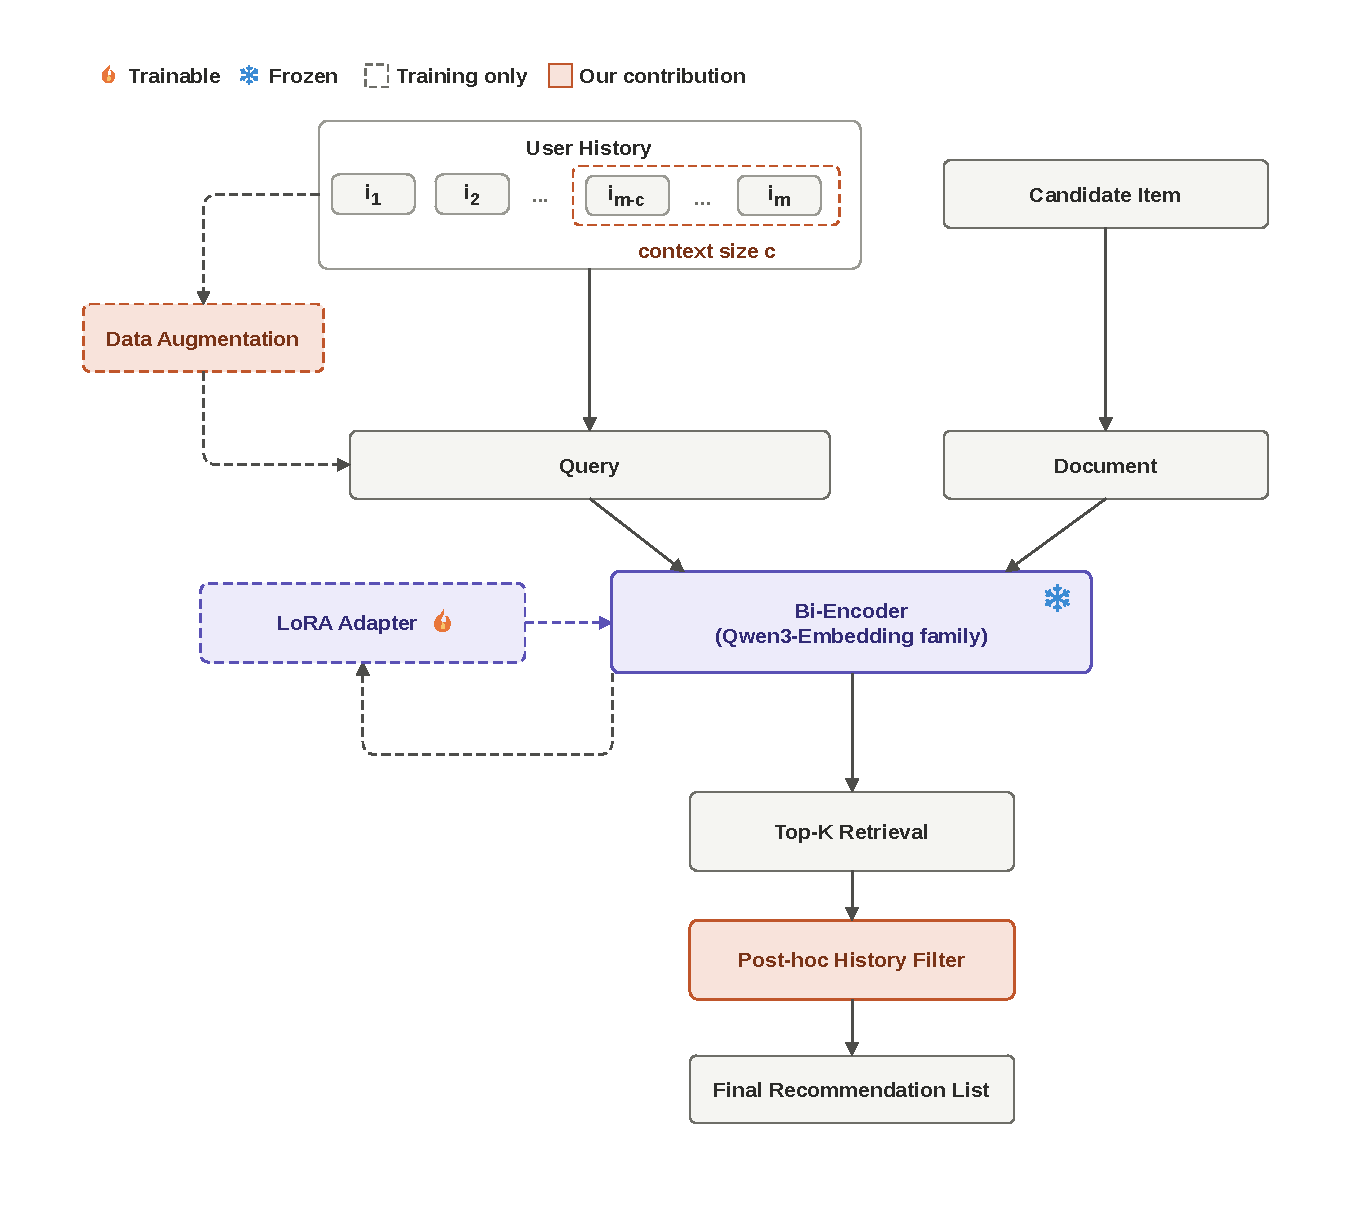
\includegraphics[width=1\linewidth]{fade_architecture.pdf}
    \caption{FADE pipeline overview}
    \label{fig:architecture}
\end{figure}

\subsection{Problem Statement}
\label{sec:problem}

Let $\mathcal{U}$ and $\mathcal{I}$ denote the sets of users and items, respectively. For each user $u \in \mathcal{U}$, the interaction history is a chronologically ordered sequence $S_u = (i_1^u,
i_2^u, \dots, i_{n_u}^u)$, $i_t^u \in \mathcal{I}$. Given a prefix $S_u^{<t} = (i_1^u, \dots,
i_{t-1}^u)$, the goal of sequential recommendation (SR) is to predict the item $i_t^u$ the user is most likely to interact with next, typically cast as ranking the full item set $\mathcal{I}$ by relevance to $S_u^{<t}$.

We reformulate this ranking problem as a text retrieval problem. Let $T: \mathcal{I} \to
\Sigma^{*}$ map each item to a short textual description (its title, in our experiments). Given a context size $c$, we define a query construction function
\[
Q(S_u^{<t}) = T(i_{t-c}^u) \,\Vert\, T(i_{t-c+1}^u) \,\Vert\, \dots \,\Vert\, T(i_{t-1}^u)
\]
that concatenates the titles of the $c$ most recent items into a single passage of text, and we treat the entire item set as a document corpus $\mathcal{D} = \{T(i) : i \in \mathcal{I}\}$, one passage per item. We build the query from only the $c$ most recent items rather than the user's entire history $S_u^{<t}$: concatenating every item a user has ever interacted with would make the query grow unboundedly with history length, quickly exceeding the backbone's context window for users with unusually long interaction histories (sequence lengths run into the hundreds for a non-trivial tail of users even in our datasets, up to 550 items; see Table~\ref{tab:datasets}) and diluting the signal relevant to the immediate next item among a large amount of older, less relevant context. The SR task then reduces to retrieving, for query $Q(S_u^{<t})$, the passage $d^{*} \in \mathcal{D}$ that maximizes similarity to the query in a learned embedding space:
\[
d^{*} = \argmax_{d \in \mathcal{D}} \; \mathrm{sim}\big(f(Q(S_u^{<t})), f(d)\big)
\]
where $f$ is a text encoder and $\mathrm{sim}(\cdot,\cdot)$ is cosine similarity. This formulation lets us reuse LLM-based dense retrieval machinery --- pretrained embedding backbones, contrastive fine-tuning, ANN search --- directly for SR, in place of item-ID embedding tables learned from scratch as in SASRec/GRU4Rec.

\subsection{Bi-Encoder}
\label{sec:biencoder}

We solve this retrieval problem with a \textbf{bi-encoder}: queries and documents are encoded independently into fixed-size vectors by a shared text encoder $f_\theta$, and relevance is scored by the cosine similarity of these vectors. This architecture follows the bi-encoder paradigm introduced by DPR~\cite{karpukhin2020} and adapted to LLM backbones by RepLLaMA~\cite{ma2024}; we describe our specific instantiation below and note where it departs from this prior work, without re-attributing every individual design choice to it. $f_\theta$ is built on a pretrained decoder-only LLM; how we adapt this backbone for training is described separately in Sect.~\ref{sec:lora}.

\paragraph{Encoding.}
Given tokenized input text $x$ --- either a query $Q$ produced by $Q(\cdot)$ or a document $D = T(i)$ for some item $i$ --- the decoder processes $x$ autoregressively under a causal self-attention mask, producing hidden states $H =
(h_1,\dots,h_L)$ for the $L$ input tokens. We take the hidden state of the final token as the text representation, $e_x = h_L$. Because the backbone is a causal decoder rather than a bidirectional encoder, $h_L$ is the only position that has attended to the entire input sequence, which is why we pool at the last token instead of prepending a [CLS] token as BERT-style dense retrievers do. The pooled vector is $\ell_2$-normalized,
\[
\hat e_x = e_x / \lVert e_x \rVert_2,
\]
and similarity between a query and a document is the cosine similarity of their normalized embeddings, $\mathrm{sim}(Q,D) = \hat e_Q \cdot \hat e_D$.

\paragraph{Tied encoder.}
The same function $f_\theta$ --- the same backbone weights and the same LoRA adapters --- encodes both queries and documents: there is no query-specific or document-specific parameter anywhere in the model, and no explicit marker distinguishes the two at the input level either; $Q(S_u^{<t})$ and $T(i)$ are both just passed through $f_\theta$ as plain text. This is a deliberate design choice rather than an oversight. The original DPR formulation trains two independently parameterized encoders, one for queries and one for passages; at LLM scale, doing the same would double an already substantial parameter and memory budget, and a sufficiently expressive backbone can plausibly infer from context alone whether it is encoding a multi-item history or a single item title, without needing separate parameters to do so.

\subsection{LoRA Adapter}
\label{sec:lora}

Fully fine-tuning $f_\theta$ would require far more compute, memory, and training time than is available on commodity hardware, so instead we adapt the backbone with \textbf{Low-Rank Adaptation (LoRA)}~\cite{hu2022}, which freezes the pretrained weights and injects a small number of trainable low-rank matrices into the backbone's attention and feed-forward projections. This leaves the vast majority of the backbone's parameters untouched while still letting it adapt to the retrieval objective, making fine-tuning practical on a single consumer GPU.

\paragraph{Training objective.}
The encoder is fine-tuned with the InfoNCE contrastive loss. For a training example consisting of query $Q_i$, one positive document $D_i^+$ (the ground-truth next item), and $g-1$ explicit negative documents (group size $g$), the loss over training batch $\mathcal{B}$ is
\[
\mathcal{L} = -\log \frac{\exp(\mathrm{sim}(Q_i, D_i^+)/\tau)}{\sum_{D \in \mathcal{B}} \exp(\mathrm{sim}(Q_i, D)/\tau)}
\]
with temperature $\tau$. $\mathcal{B}$ contains the explicit negatives paired with $Q_i$ as well as the positive and negative documents of every other query in the batch (in-batch negatives), following standard dense-retrieval training practice.

\subsection{Data Augmentation}
\label{sec:augmentation}

Under the standard leave-one-out protocol, the last item of $S_u$ is held out for testing, the second-to-last for validation, and the remaining prefix $S_u^{\text{train}} = (i_1^u, \dots,
i_m^u)$ ($m = n_u - 2$) is used for training. In its simplest form this produces exactly \textbf{one} training pair per user: query $Q(S_u^{\text{train}})$, built from the $c$ items
immediately preceding $i_m^u$, paired with positive $D^+ = T(i_m^u)$.

This severely underuses the available supervision relative to causal sequence models. SASRec, for instance, applies a causal self-attention mask over the entire training sequence and is supervised to predict $i_{t+1}$ from $i_{1:t}$ \emph{at every position} $t$ in a single forward pass --- effectively obtaining $m-c$ (context, next-item) pairs ``for free'' from one sequence. Our bi-encoder has no equivalent mechanism: without intervention, each user contributes only one gradient signal per epoch, which is especially limiting for users with long histories and for corpora with many users but comparatively few items relating them.

We recover this missing supervision explicitly via sliding-window augmentation, adapted from the sub-session splitting technique commonly used in session-based recommendation. For each user, we slide a window of size $c$ across $S_u^{\text{train}}$ and emit one training pair per valid position $t \in \{c+1,\dots,m\}$:
\[
Q_t = Q\big((i_{t-c}^u,\dots,i_{t-1}^u)\big), \qquad D_t^+ = T(i_t^u)
\]
yielding up to $m-c$ pairs per user instead of one, while preserving chronological order within each window (the underlying sequence is never shuffled).

\subsection{History Filter}
\label{sec:filter}
At inference time, given query $Q(S_u^{<t})$, the retriever ranks the entire corpus $\mathcal{D}$ by similarity and returns the top-$K$ candidates via approximate nearest-neighbor search (FAISS); as discussed in Sect.~\ref{sec:intro}, this ranked list is heavily biased toward items the user has already consumed. We attribute this to the training objective rather than to any explicit preference for ``popular'' or ``similar'' items: because $D_i^+$ is always the \emph{next}, previously-unseen item, the contrastive loss never constructs a negative pair whose text is verbatim (or near-verbatim) contained in the query itself. Consequently, nothing in training penalizes assigning maximal similarity to a candidate whose text overlaps almost completely with the query, exactly the case when the candidate is one of the $c$ items making up the query's own context window. At inference, the model reproduces this shortcut: an item's own presence in the query is itself powerful evidence of ``relevance'' to the trained similarity function, regardless of whether re-recommending it is desirable.

We fix this without any additional training via a \textbf{history filter}: after retrieving the top-$K$ ranked list for a query, we remove every item the user has interacted with prior to position $t$, namely the user's entire interaction history $S_u^{<t}$ and not merely the $c$ items forming the query's own context window, and re-rank the remaining candidates before producing the final recommendation. The filter requires no retraining and no GPU: it operates directly on already-computed FAISS rankings, making it essentially free to apply.

\section{Experiments}
\label{sec:experiments}
\subsection{Datasets}
\label{sec:datasets}
We evaluate FADE on three public datasets, all Amazon (2014) product categories~\cite{mcauley2015} widely
used as SR benchmarks in prior LLM-based work: \textbf{Beauty}, \textbf{Sports and Outdoors}, and
\textbf{Toys and Games}. Table~\ref{tab:datasets} summarizes their statistics.

\begin{table}[H]
\centering
\caption{Dataset statistics.}
\label{tab:datasets}
\begin{tabular}{lrrrrr}
\toprule
Dataset & Users & Items & Interactions & Avg.\ seq.\ len & Max seq.\ len \\
\midrule
Amazon Beauty              & 22{,}363 & 12{,}101 & 198{,}502 & 8.9 & 204 \\
Amazon Sports and Outdoors & 35{,}598 & 18{,}357 & 296{,}337 & 8.3 & 296 \\
Amazon Toys and Games      & 19{,}412 & 11{,}924 & 167{,}597 & 8.6 & 550 \\
\bottomrule
\end{tabular}
\end{table}

Following standard practice in the SR literature, each dataset is 5-core filtered (every user and item has at least 5 interactions) and split with the leave-one-out protocol: for each user, the last interaction is held out for testing, the second-to-last for validation, and the remaining prefix is used for training. At both validation and test time we rank the \emph{entire} item set rather than a sampled subset of negatives, since sampled-negative evaluation is known to produce rankings of methods that do not always agree with full-ranking evaluation.

\subsection{Experimental Setup}
\label{sec:setup}
We use the \textbf{Qwen3-Embedding} family as the backbone for FADE. We choose Qwen3-Embedding over a general-purpose, generation-oriented LLM because its pretraining objective is already aligned with what our retriever needs to do: represent a piece of text as a single vector that can be compared against other such vectors, rather than predict a distribution over the next token. We report results at two backbone sizes, 0.6B and 4B; which of the two we adopt as FADE's headline backbone is a decision we defer until results for both are complete across all three datasets. Both backbone sizes are adapted with LoRA (rank $r=16$, scaling $\alpha=64$, dropout $0.1$) injected into the query, key, value, output, gate, up-, and down-projection matrices of every transformer block. We fine-tune with the InfoNCE objective at temperature $\tau=0.01$, using Tevatron v2 with DeepSpeed ZeRO-2, a learning rate of $1\times10^{-4}$, and 3 training epochs. All FADE experiments run on a single NVIDIA RTX~3090 24GB VRAM.

The ID-based baselines that we reproduce ourselves (GRU4Rec, SASRec, SR-GNN) are trained with RecBole 1.2.1 under a protocol matched as closely as possible to FADE's: full-softmax cross-entropy loss (no negative sampling during training) and \texttt{MAX\_ITEM\_LIST\_LENGTH=200}.

\subsection{Evaluation Metrics}
\label{sec:metrics}
We report Normalized Discounted Cumulative Gain (NDCG@$K$) and Hit Ratio (HR@$K$ --- equivalent to Recall@$K$ since each test instance has exactly one relevant item), at $K \in \{5,10,20\}$:
\begin{itemize}
\item \textbf{HR@$K$}: the fraction of test instances for which the held-out item appears in the top-$K$ ranked list.
\item \textbf{NDCG@$K$}: the average, over test instances, of $1/\log_2(\mathrm{rank}+1)$ when the held-out item is ranked within the top $K$ (and $0$ otherwise) --- rewarding a hit at rank~1 more than an equally-counted hit at rank~$K$, unlike HR@$K$.
\end{itemize}

\subsection{Baseline Methods}
\label{sec:baselines}
We compare against two groups of baselines, together with a zero-shot lower bound.

\textbf{ID-based sequential models} represent items with trainable ID embeddings and require no textual side information: GRU4Rec~\cite{hidasi2016} (RNN-based), SR-GNN~\cite{wu2019} (graph-based), and SASRec~\cite{kang2018} (self-attention, causal). We reproduce all three ourselves under the protocol in Sect.~\ref{sec:setup}.

\textbf{LLM- and generative-retrieval-based models}, for which we report literature numbers rather than reproducing them ourselves (Sect.~\ref{sec:results} states exactly which numbers in each table come from which source): TIGER~\cite{rajput2023} (generates a discrete Semantic ID for the target item), ActionPiece~\cite{hou2025} (improves TIGER's tokenization with co-occurrence-aware token merging), EAGER-LLM~\cite{hong2025} (injects collaborative signals into a decoder-only LLM recommender), LlamaRec~\cite{yue2023} (re-ranks a separate candidate retriever's output via an LLM verbalizer), P5~\cite{geng2022} (casts recommendation as a unified text-to-text objective), E4SRec~\cite{li2024} (uses an LLM as a sequence encoder feeding an ID-embedding prediction head), and GLoSS-8B, the 8B-parameter variant of GLoSS~\cite{acharya2025} (a generate-then-retrieve dense-retrieval pipeline).

Finally, we report a \textbf{zero-shot} lower bound: the untuned Qwen3-Embedding-0.6B backbone used directly as a retriever without any fine-tuning, to quantify how much of FADE's performance comes from fine-tuning versus from the pretrained backbone alone.

\subsection{Overall Results}
\label{sec:results}

Table~\ref{tab:beauty} reports NDCG and HR at $K \in \{5,10\}$ on all three datasets, with the best result in each column in \textbf{bold} (left blank where an entry is not yet available). Methods marked \textdagger{} are literature-reported numbers, copied from their respective papers rather than reproduced by us; unmarked methods (SR-GNN, FADE) are reproduced by us under the protocol in Sect.~\ref{sec:setup} on every dataset. For Toys and Games specifically, GRU4Rec and SASRec are also reproduced by us rather than literature-reported, since we have not verified literature baseline numbers for these two specifically on this dataset, so \textdagger{} on these two rows applies only to their Beauty/Sports columns. TIGER, P5, E4SRec, and GLoSS-8B all report results on Toys and Games in their original papers under the same 5-core, leave-one-out protocol, and we copy those numbers directly (verified against the original papers; GLoSS-8B, like on Beauty/Sports, reports only Recall@5/NDCG@5, not the @10 metrics). ActionPiece and EAGER-LLM do not evaluate on Toys and Games at all in their original papers --- ActionPiece uses CDs and Vinyl as its third dataset instead of Toys, and EAGER-LLM uses Musical Instruments --- so their Toys and Games cells are left blank rather than substituted with a number from a different dataset; LlamaRec's Toys and Games numbers have not been verified at the time of writing and are likewise left blank.
\begin{table}[H]
\centering
\caption{Beauty, Sports and Outdoors, and Toys and Games. R = Recall, N = NDCG; \textdagger{} = literature-reported; \emph{TBD} = training in progress at time of writing; -- = not reported/not verified for this dataset.}
\label{tab:beauty}
\tiny
\setlength{\tabcolsep}{2pt}
\begin{tabular}{lcccccccccccc}
\toprule
& \multicolumn{4}{c}{Beauty} & \multicolumn{4}{c}{Sports and Outdoors} & \multicolumn{4}{c}{Toys and Games} \\
\cmidrule(lr){2-5} \cmidrule(lr){6-9} \cmidrule(lr){10-13}
Method & R@5 & R@10 & N@5 & N@10 & R@5 & R@10 & N@5 & N@10 & R@5 & R@10 & N@5 & N@10 \\
\midrule
GRU4Rec\textdagger{}& 0.0164 & 0.0283 & 0.0099 & 0.0137 & 0.0129 & 0.0204 & 0.0086 & 0.0110 & 0.0352 & 0.0522 & 0.0247 & 0.0301 \\
SASRec\textdagger{}& 0.0387 & 0.0605 & 0.0249 & 0.0318 & 0.0233 & 0.0350 & 0.0154 & 0.0192 & 0.0600 & 0.0877 & 0.0343 & 0.0433 \\
SR-GNN      & 0.0363 & 0.0552 & 0.0252 & 0.0312 & 0.0200 & 0.0310 & 0.0130 & 0.0165 & 0.0332 & 0.0476 & 0.0237 & 0.0283 \\
TIGER\textdagger{}       & 0.0454 & 0.0648 & 0.0321 & 0.0384 & 0.0264 & 0.0400 & 0.0181 & 0.0225 & 0.0521 & 0.0712 & 0.0371 & 0.0432 \\
ActionPiece\textdagger{} & 0.0511 & --     & 0.0340 & --     & 0.0316 & --     & 0.0205 & --     & -- & -- & -- & -- \\
EAGER-LLM\textdagger{}   & 0.0548 & 0.0830 & 0.0369 & 0.0459 & 0.0373 & 0.0569 & 0.0251 & 0.0315 & -- & -- & -- & -- \\
LlamaRec\textdagger{}    & 0.0852 & 0.1524 & 0.0543 & 0.0759 & --     & --     & --     & --     & -- & -- & -- & -- \\
P5\textdagger{}          & 0.0503 & --     & 0.0370 & --     & 0.0272 & --     & 0.0169 & --     & 0.0648 & 0.0709 & 0.0567 & 0.0587 \\
E4SRec\textdagger{}      & 0.0525 & --     & 0.0360 & --     & 0.0281 & --     & 0.0196 & --     & 0.0566 & 0.0798 & 0.0405 & 0.0479 \\
GLoSS-8B\textdagger{}    & 0.0681 & --     & 0.0442 & --     & 0.0364 & --     & 0.0238 & --     & 0.0796 & -- & 0.0529 & -- \\
\textbf{FADE-0.6B} & \textbf{0.0730} & \textbf{0.1088} & \textbf{0.0501} & \textbf{0.0616} & \textbf{0.0447} & \textbf{0.0684} & \textbf{0.0294} & \textbf{0.0371} & \textbf{0.0869} & \textbf{0.1273} & \textbf{0.0592} & \textbf{0.0722} \\
FADE-4B     & 0.0728 & 0.1083 & 0.0497 & 0.0611 & \emph{TBD} & \emph{TBD} & \emph{TBD} & \emph{TBD} & \emph{TBD} & \emph{TBD} & \emph{TBD} & \emph{TBD} \\
\bottomrule
\end{tabular}
\end{table}
On Beauty and Sports, FADE-0.6B achieves the best NDCG@10 and HR@10 of every method compared, beating the strongest ID-based baseline (SASRec) by +93.7\% and +93.2\% NDCG@10 respectively, and beating every LLM/generative-retrieval baseline as well --- including GLoSS-8B, an 8B-parameter model, despite FADE-0.6B having less than a tenth as many parameters.

On Toys and Games, FADE-0.6B likewise achieves the best NDCG@10 and HR@10 of every method compared, now that the self-reproduced GRU4Rec/SASRec/SR-GNN baselines for this dataset have finished training. It beats the strongest ID-based baseline (SASRec) by +45.2\% HR@10 and +66.7\% NDCG@10, and beats every verified LLM/generative-retrieval baseline as well, by margins ranging from +4.4\% (NDCG@5 over P5) to +59.5\% (HR@10 over E4SRec). Unlike on Beauty and Sports, where SASRec is also the strongest ID-based baseline, GRU4Rec and SR-GNN trail SASRec by a wide margin on Toys and Games rather than approaching or exceeding it. FADE-4B has not yet been trained on this dataset; we leave that comparison for the camera-ready version.

\subsection{Ablation Study}
\label{sec:ablation}
Table~\ref{tab:ablation} ablates FADE on all three datasets, using the 0.6B backbone, by removing one component at a time: \textbf{``$-$ History filter''} uses the raw FAISS ranking unmodified instead of applying the filter; \textbf{``$-$ Augmentation''} removes sliding-window augmentation from training; and \textbf{``Zero-shot (+ filter)''} fine-tunes nothing at all but still applies the history filter at inference, isolating the contribution of fine-tuning itself from that of the filter (the fully raw zero-shot number, without the filter, is lower still and is omitted here for space).

\begin{table}[H]
\centering
\caption{Ablation study (NDCG@10 / R@10).}
\label{tab:ablation}
\footnotesize
\begin{tabular}{lcccccc}
\toprule
& \multicolumn{2}{c}{Beauty} & \multicolumn{2}{c}{Sports} & \multicolumn{2}{c}{Toys and Games} \\
\cmidrule(lr){2-3} \cmidrule(lr){4-5} \cmidrule(lr){6-7}
Variant & NDCG@10 & R@10 & NDCG@10 & R@10 & NDCG@10 & R@10 \\
\midrule
\textbf{FADE (full)}    & \textbf{0.0616} & \textbf{0.1088} & \textbf{0.0371} & \textbf{0.0684} & \textbf{0.0722} & \textbf{0.1273} \\
$-$ History filter      & 0.0390 & 0.0905 & 0.0260 & 0.0574 & 0.0471 & 0.1057 \\
$-$ Augmentation        & 0.0581 & 0.1019 & 0.0279 & 0.0523 & 0.0608 & 0.1082 \\
Zero-shot (+ filter)    & 0.0202 & 0.0364 & 0.0102 & 0.0195 & 0.0244 & 0.0461 \\
\bottomrule
\end{tabular}
\end{table}

Removing the history filter is consistently the single largest drop among the two components we ablate: NDCG@10 falls by 36.7\% on Beauty, 29.9\% on Sports, and 34.8\% on Toys and Games when the raw FAISS ranking is used unmodified --- the direct empirical counterpart to the bias introduced in Sects.~\ref{sec:intro} and \ref{sec:filter}. Removing augmentation also hurts substantially, though its effect size varies more across datasets (5.7\% on Beauty vs.\ 24.8\% on Sports and 15.8\% on Toys and Games). Removing fine-tuning entirely (zero-shot) is by far the largest drop of all --- 66--73\% NDCG@10 depending on dataset --- confirming that most of FADE's performance comes from adapting the backbone to the retrieval objective, not from the pretrained embedding space alone.

\subsection{Effect of Context Size}
\label{sec:context}
The context size $c$ (Sect.~\ref{sec:problem}) controls how many of the most recent items are concatenated into the query. Sweeping $c$ with augmentation enabled would require re-generating the augmented training set and re-encoding the full corpus for every value of $c$, which is expensive; we therefore run this sweep with augmentation disabled, holding every other setting fixed at the values in Sect.~\ref{sec:setup} (group size 32, 3 training epochs), for $c \in \{1,2,3,4,5\}$ on all three datasets. Table~\ref{tab:context} reports NDCG@10 and Recall@10 after applying the history filter, with the best $c$ per dataset/metric in \textbf{bold}. Because augmentation is off, these numbers are not directly comparable to the main FADE-0.6B results in Table~\ref{tab:beauty}; they isolate the effect of $c$ on its own.

\begin{table}[H]
\centering
\caption{Effect of context size $c$ on NDCG@10 / R@10, no augmentation, history filter applied.}
\label{tab:context}
\footnotesize
\begin{tabular}{lcccccc}
\toprule
& \multicolumn{2}{c}{Beauty} & \multicolumn{2}{c}{Sports} & \multicolumn{2}{c}{Toys and Games} \\
\cmidrule(lr){2-3} \cmidrule(lr){4-5} \cmidrule(lr){6-7}
$c$ & NDCG@10 & R@10 & NDCG@10 & R@10 & NDCG@10 & R@10 \\
\midrule
1 & 0.0561 & 0.0958 & 0.0287 & 0.0521 & \textbf{0.0632} & 0.1062 \\
2 & 0.0573 & 0.0982 & 0.0297 & \textbf{0.0559} & 0.0630 & 0.1086 \\
3 & \textbf{0.0574} & \textbf{0.1014} & \textbf{0.0298} & 0.0551 & 0.0621 & 0.1104 \\
4 & 0.0556 & 0.0980 & 0.0290 & 0.0554 & 0.0610 & 0.1098 \\
5 & 0.0543 & 0.0979 & 0.0295 & 0.0552 & 0.0620 & \textbf{0.1105} \\
\bottomrule
\end{tabular}
\end{table}

The spread between the best and worst $c$ in this range is modest --- 5.7\% NDCG@10 on Beauty, 3.8\% on Sports, 3.6\% on Toys and Games --- so FADE-0.6B (without augmentation) is relatively robust to this choice for $c \in \{1,\dots,5\}$. No single $c$ dominates across all datasets and metrics: Beauty and Sports both peak at $c=3$ on NDCG@10, whereas Toys and Games peaks at the smallest value, $c=1$, on NDCG@10 but at the largest, $c=5$, on Recall@10. We do not observe the monotonic ``more context is better'' trend one might expect from a longer query carrying more information; if anything, Beauty and Sports show a mild inverted-U shape, degrading slightly again after $c=3$.

\section{Conclusion}
\label{sec:conclusion}

We presented FADE, a bi-encoder retriever that reformulates sequential recommendation as dense retrieval over item text. Applying this reformulation to SR raises three challenges that FADE addresses directly: encoding an entire item set with a bi-encoder rather than an infeasible cross-encoder; recovering the per-position supervision that the standard leave-one-out protocol does not provide, through sliding-window data augmentation; and correcting seen-item bias, a tendency for previously-consumed items to dominate the ranked list, through a lightweight, training-free history filter.

Across all three datasets, FADE-0.6B substantially outperforms strong ID-based baselines (SASRec, GRU4Rec, SR-GNN); on Beauty and Sports it also beats every prior LLM-based recommender we compare against, including an 8B-parameter dense-retrieval baseline despite having less than a tenth as many parameters, and on Toys and Games it beats every one of those baselines for which we could verify literature numbers. Results for the larger FADE-4B backbone on Toys and Games were not yet available at the time of writing and are left for the camera-ready version. Our ablation study, run across all three datasets, confirms that both the history filter and sliding-window augmentation contribute substantially to FADE's performance, with most of the overall gain coming from fine-tuning the backbone itself.

%
\begin{credits}
\subsubsection{\ackname}
% TODO: điền grant/funding nếu có, hoặc xoá mục này nếu không có acknowledgment.
This study was partially supported by MLA Lab, PTIT..

\end{credits}
%
% ---- Bibliography ----
%
\begin{thebibliography}{19}

\bibitem{hidasi2016}
Hidasi, B., Karatzoglou, A., Baltrunas, L., Tikk, D.: Session-based Recommendations with Recurrent
Neural Networks. In: ICLR (2016)

\bibitem{wu2019}
Wu, S., Tang, Y., Zhu, Y., Wang, L., Xie, X., Tan, T.: Session-based Recommendation with Graph
Neural Networks. In: AAAI. vol.~33(1), pp. 346--353 (2019)

\bibitem{kang2018}
Kang, W.C., McAuley, J.: Self-Attentive Sequential Recommendation. In: ICDM (2018)

\bibitem{karpukhin2020}
Karpukhin, V., O\u{g}uz, B., Min, S., Lewis, P., Wu, L., Edunov, S., Chen, D., Yih, W.: Dense
Passage Retrieval for Open-Domain Question Answering. In: EMNLP. pp. 6769--6781 (2020)

\bibitem{ma2024}
Ma, X., Wang, L., Yang, N., Wei, F., Lin, J.: Fine-Tuning LLaMA for Multi-Stage Text Retrieval. In:
SIGIR '24. pp. 2421--2425 (2024)

\bibitem{hu2022}
Hu, E.J., Shen, Y., Wallis, P., Allen-Zhu, Z., Li, Y., Wang, S., Wang, L., Chen, W.: LoRA:
Low-Rank Adaptation of Large Language Models. In: ICLR (2022)

\bibitem{mcauley2015}
McAuley, J., Targett, C., Shi, Q., van den Hengel, A.: Image-based Recommendations on Styles and
Substitutes. In: SIGIR. pp. 43--52 (2015)

\bibitem{rajput2023}
Rajput, S., Mehta, N., Singh, A., Hulikal Keshavan, R., Vu, T., Heldt, L., Hong, L., Tay, Y., Tran,
V., Samost, J., Kula, M., Chi, E.H., Sathiamoorthy, M.: Recommender Systems with Generative
Retrieval. In: NeurIPS (2023)

\bibitem{hou2025}
Hou, Y., Ni, J., He, Z., Sachdeva, N., Kang, W.C., Chi, E.H., McAuley, J., Cheng, D.Z.:
ActionPiece: Contextually Tokenizing Action Sequences for Generative Recommendation. In: ICML
(2025)

\bibitem{hong2025}
Hong, M., Xia, Y., Wang, Z., Zhu, J., Wang, Y., Cai, S., Yang, X., Dai, Q., Dong, Z., Zhang, Z.,
Zhao, Z.: EAGER-LLM: Enhancing Large Language Models as Recommenders through Exogenous
Behavior-Semantic Integration. In: WWW '25. pp. 2754--2762 (2025)

\bibitem{yue2023}
Yue, Z., Rabhi, S., de Souza Pereira Moreira, G., Wang, D., Oldridge, E.: LlamaRec: Two-Stage
Recommendation using Large Language Models for Ranking. In: PGAI Workshop @ CIKM (2023)

\bibitem{geng2022}
Geng, S., Liu, S., Fu, Z., Ge, Y., Zhang, Y.: Recommendation as Language Processing (RLP): A
Unified Pretrain, Personalized Prompt \& Predict Paradigm (P5). In: RecSys. pp. 299--315 (2022)

\bibitem{li2024}
Li, X., Chen, C., Zhao, X., Zhang, Y., Xing, C.: E4SRec: An Elegant Effective Efficient Extensible
Solution of Large Language Models for Sequential Recommendation. In: WWW '24 (2024)

\bibitem{acharya2025}
Acharya, K., Petrov, A.V., Ziani, J.: Generative Language Models with Semantic Search for
Sequential Recommendation. In: Online and Adaptive Recommender Systems (OARS) Workshop @ KDD
(2025)

\bibitem{wang2022e5}
Wang, L., Yang, N., Huang, X., Jiao, B., Yang, L., Jiang, D., Majumder, R., Wei, F.: Text
Embeddings by Weakly-Supervised Contrastive Pre-training. arXiv:2212.03533 (2022)

\bibitem{tan2016}
Tan, Y.K., Xu, X., Liu, Y.: Improved Recurrent Neural Networks for Session-based Recommendations.
In: Workshop on Deep Learning for Recommender Systems (DLRS) @ RecSys (2016)

\bibitem{tang2018}
Tang, J., Wang, K.: Personalized Top-N Sequential Recommendation via Convolutional Sequence
Embedding. In: WSDM. pp. 565--573 (2018)

\bibitem{yu2021}
Yu, S., Liu, Z., Xiong, C., Feng, T., Liu, Z.: Few-Shot Conversational Dense Retrieval. In: SIGIR
'21. pp. 829--838 (2021)

\bibitem{yi2019}
Yi, X., Yang, J., Hong, L., Cheng, D.Z., Heldt, L., Kumthekar, A., Zhao, Z., Wei, L., Chi, E.:
Sampling-Bias-Corrected Neural Modeling for Large Corpus Item Recommendations. In: RecSys '19. pp.
269--277 (2019)

\end{thebibliography}
\end{document}
